% Copyright 2009 by Tomasz Mazur
%
% This file may be distributed and/or modified in all ways.


\documentclass[xcolor=pdftex,t,11pt]{beamer}

%%%%%%%%%%%%%%%%%%%%%%%%%%%%%%%%%%
%       SET OPTIONS BELOW        %
%%%%%%%%%%%%%%%%%%%%%%%%%%%%%%%%%%

\usetheme[
% Toggle showing page counter
pagecounter=true,
%
% String to be used between the current page and the
% total page count, e.g. of, /, from, etc.
pageofpages=of,
%
% Defines the shape of bullet points. Available options: circle, square
bullet=circle,
%
% Show a line below the frame title. 
titleline=true,
%
% Set the style of the title page (true for fancy, false for standard)
alternativetitlepage=true,
%
% Institution logo for fancy title page.
% Comment out to remove the logo from the title page.
% IMPORTANT: THERE IS A BUG IN SOME VERSIONS OF PDFLATEX AND FONTS
% ON THE LOGOS ARE NOT RENDERED PROPERLY. IN SUCH A CASE ADD `2` 
% TO THE NAME OF THE LOGO, E.G. comlab2 INSTEAD OF comlab
%titlepagelogo=images/titlepage/ou,
%
% Department footer logo for fancy title page
% Comment out to remove the logo from the footer of the title page/
% IMPORTANT: THERE IS A BUG IN SOME VERSIONS OF PDFLATEX AND FONTS
% ON THE LOGOS ARE NOT RENDERED PROPERLY. IN SUCH A CASE ADD `2` 
% TO THE NAME OF THE LOGO, E.G. comlab2 INSTEAD OF comlab
%titlepagefooterlogo=images/titlepage/comlab,
%
% Institution/department logo for ordinary slides
% Comment this line out to remove the logo from all the pages.
% Available logos are: ou, comlab, comlabinline, comlabou
% IMPORTANT: THERE IS A BUG IN SOME VERSIONS OF PDFLATEX AND FONTS
% ON THE LOGOS ARE NOT RENDERED PROPERLY. IN SUCH A CASE ADD `2` 
% TO THE NAME OF THE LOGO, E.G. comlab2 INSTEAD OF comlab
%ordinarypageslogo=TU-Signet,
%
%
% Add watermark in the bottom right corner
%watermark=<filename>,
%
% Set the height of the watermark.
%watermarkheight=100pt,
%
% The watermark image is 4 times bigger than watermarkheight.
%watermarkheightmult=4,
]{Torino}

% Select color theme. Available options are:
% mininmal, greenandblue, blue, red
\usecolortheme{blue}

%Select different font themes.Available options are:
% default, serif, structurebold, structureitalicserif, structuresmallcapsserif
\usefonttheme{structurebold}



\usepackage{tikz}
\usepackage{pgf}
\usepackage{dot2texi}

%\usepackage[pdftex]{graphicx}
\usepackage{graphviz}


\pgfdeclareimage[height=6ex]{ou-logo}{images/ou}

\logo{\pgfuseimage{ou-logo}}

\usepackage{listings}

\lstset{language=C,
 basicstyle=\tiny
 }

\usepackage{ifthen}

\usepackage{moreverb}
\usepackage{pgf}
\usepackage{tikz}
\usetikzlibrary{arrows, automata, shapes.multipart, chains, positioning, fit, calc}

\usepackage{pifont}
\newcommand{\xmark}{\ding{55}}

\usepackage{color}
\definecolor{light-gray}{gray}{0.80}

\lstset{escapeinside={<@}{@>}}

\definecolor{tachameleon}{rgb}{0.54118, 0.88627, 0.20392}       % #8ae234
\definecolor{ta2chameleon}{rgb}{0.45098, 0.82353, 0.086275}     % #73d216
\definecolor{ta3chameleon}{rgb}{0.30588, 0.60392, 0.023529}     % #4e9a06


\newcommand{\red}[1]{\textcolor{red}{#1}}
\newcommand{\blue}[1]{\textcolor{blue}{#1}}
\newcommand{\green}[1]{\textcolor{ta3chameleon}{#1}}



%%%%%%%%%%%%%%%%%%%%%%%%%%%%%%%%%%
%       PRESENTATION INFO        %
%%%%%%%%%%%%%%%%%%%%%%%%%%%%%%%%%%

\author{Cristina David \and Daniel Kroening \and Matt Lewis}
\title{Unrestricted Termination and Non-Termination Arguments for Bit-Vector Programs}
%\subtitle{}
\institute{University of Oxford}
\date{\today}

\begin{document}



%%%%%%%%%%%%%%%%%%%%%%%%%%%%%%%%%%
%       SLIDE DEFINITIONS        %
%%%%%%%%%%%%%%%%%%%%%%%%%%%%%%%%%%

\begin{frame}[plain]
  \titlepage
\end{frame}

\begin{frame}{Outline}
  \tableofcontents
\end{frame}

\section{What's The Problem?}
\begin{frame}[fragile]{Motivation}
Does this program terminate?
\begin{center}
\begin{minipage}{0.4\linewidth}
 \begin{lstlisting}[language=C,basicstyle=\normalsize]
while (x > 0) {
  x++;
}
 \end{lstlisting}
\end{minipage}
\end{center}

\pause

That depends...

It \emph{does not} terminate if the program operates on integers...

But it \emph{does} terminate if the program operates on fixed-width words
(-x decreases monotonically and is bounded by -MAXINT).

\end{frame}

\begin{frame}[fragile]{Motivation}
Which of these guys terminates?
\begin{center}
\begin{minipage}{0.45\linewidth}
 \begin{lstlisting}[language=C,basicstyle=\normalsize]
while (x > 0) {
  x = (x - 1) & x;
}
\end{lstlisting}
\end{minipage}
\begin{minipage}{0.45\linewidth}
 \begin{lstlisting}[language=C,basicstyle=\normalsize]
while (x > 0) {
  x = (x + 1) & x;
}
\end{lstlisting}
\end{minipage}
\end{center}

\pause

The left one does (x decreases monotonically), but the right one doesn't ($2 \rightarrow 2 \rightarrow \dots$).
\end{frame}

\begin{frame}[fragile]{Motivation}
Which of these guys terminates?
\begin{center}
\begin{minipage}{0.45\linewidth}
 \begin{lstlisting}[language=C,basicstyle=\normalsize]
while (x > 0) {
  x = x * 2;
}
\end{lstlisting}
\end{minipage}
\begin{minipage}{0.45\linewidth}
 \begin{lstlisting}[language=C,basicstyle=\normalsize]
while (x > 0) {
  x = x * 3;
}
\end{lstlisting}
\end{minipage}
\end{center}

\pause

The left one does (the position of the leftmost 1 bit increases up to a bound of 32), but the right one doesn't (if $x$ is odd to begin with, it will be odd forever).
\end{frame}


\begin{frame}{Motivation}
Proving program termination has been a big deal for a while.

\vspace{1em}

It's still quite hard to do for the programs that people write, which use bitvectors and all kinds of nonsense.
\end{frame}


\subsection{Bitvectors Are Hard}

\begin{frame}[fragile]{Bitvector Termination}
 \begin{columns}[c]
  \column{.45\textwidth}
  \emph{If a program terminates for integers, it terminates for bitvectors.}

  \uncover<2->{{\centering \color{red} \Huge \xmark
  
  }
  
  \lstinputlisting[language=C,basicstyle=\normalsize,mathescape]{term1.c}
  }

  \column{.45\textwidth}
  \emph{If a program terminates for bitvectors, it terminates for integers.}

  \uncover<3->{{\centering \color{red} \Huge \xmark
  
  }
  
  \lstinputlisting[language=C,basicstyle=\normalsize]{term2.c}
  }
 \end{columns}

 \vspace{1.5em}
 
 \uncover<4->{\Large \centering Integer and bitvector termination are incomparable!
 
 }
 
\end{frame}


\begin{frame}{Bitvector Termination}
\begin{quote}
 ``People really don't *think* about termination using bitvector arguments''
   \hspace*\fill{\small--- Anonymous Reviewer}
\end{quote}
\end{frame}


\subsection{Non-Linearity Is Hard}



\begin{frame}{Example}
\end{frame}

\section{Our Solution}

\subsection{Existential Second-Order Logic}

\begin{frame}[fragile]{Our Theory}
 We will try to build termination proofs by solving \emph{second-order constraints}.

 \vspace{1em}

 Specifically, we will build constraints of the form:

 \begin{center}
 \begin{columns}
  \column{.15\textwidth}
  $\exists \red{F} . \forall \vec{\blue{x}} . \green{\phi}(\red{F}, \vec{\blue{x}})$

  \column{.4\textwidth}
  \begin{minipage}{\textwidth}
 \begin{itemize}
  \item[$\red{F}$] a function.
  \item[$\green{\phi}$] a quantifier free formula.
  \item[$\vec{\blue{x}}$] the program variables.
 \end{itemize}
 \end{minipage}
 \end{columns}

 \end{center}

 \vspace{.75em}

 These constraints can be solved using an EPR solver (such as the one in Z3), or by using a program
 synthesiser to synthesise $\red{F}$.
\end{frame}


\begin{frame}[fragile]{Modelling Loops}
 For ease of presentation, we will consider loops of the following form:

 \begin{center}
 \begin{columns}[c]
  \column{.15\textwidth}
  \begin{minipage}{\linewidth}
 \begin{lstlisting}[language=C,basicstyle=\normalsize]
<@\red{P}@>;

while (<@\green{G}@>) {
  <@\blue{B}@>;
}
 \end{lstlisting}
 \end{minipage}
 
 \column{.4\textwidth}

 \begin{minipage}{\linewidth}
 \begin{itemize}
  \item[\red{P}] the prefix to the loop.
  \item[\green{G}] the loop guard.
  \item[\blue{B}] the loop body.
 \end{itemize}
 \end{minipage}
 \end{columns}

 \end{center}

\vspace{1em}
 
In our logical encoding, we model \green{G} as a predicate $\green{G}(x)$. \red{P} and \blue{B} are modelled as transition
relations $\red{P}(x, x')$ and $\blue{B}(x, x')$.
 
\end{frame}

\begin{frame}[fragile]{Loop Encoding Example}

\begin{columns}[c]
 \column{.5\textwidth}

 \begin{center}
 \begin{tabular}{c}

 \begin{lstlisting}[language=C,basicstyle=\normalsize,mathescape]
<@\red{x = 0}@>;

while (<@\green{x $>$ 0}@>) {
  <@\blue{x++}@>;
}
 \end{lstlisting}
 \end{tabular}
 \end{center}

 \column{.5\textwidth}
\begin{align*}
 \red{P} = & \{ (x, x') \mid x' = 0 \} \\
 \green{G} = & \{ x \mid x > 0 \} \\
 \blue{B} = & \{ (x, x') \mid x' = x + 1 \}
\end{align*}
\end{columns}

\end{frame}



\subsection{Ranking Functions: Proofs of Termination}

\begin{frame}[fragile]{Ranking Functions}
 To prove that a loop $(P, G, B)$ terminates, we will try to find a \emph{ranking function} $R$.
 
 \vspace{1em}
 
 A ranking function is some function that decreases on each loop iteration, but which cannot decrease forever.
 
%  \vspace{1em}
%  
%  A function $R$ is a ranking function for the loop $(P, G, B)$ iff it satisfies the following criteria:
%  \begin{align*}
%   \forall x . G(x) \Rightarrow & R(x) > 0 \\
%   \forall x, x' . G(x) \wedge B(x, x') \Rightarrow & R(x) > R(x')
%  \end{align*}
\end{frame}

\begin{frame}[fragile]{Ranking Functions}

\begin{center}
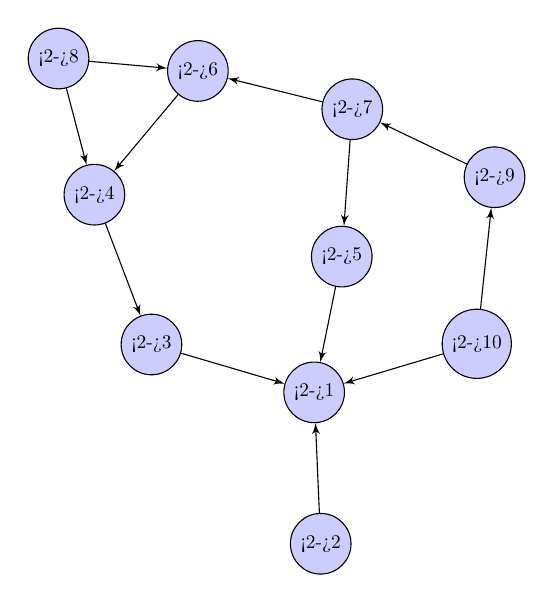
\begin{tikzpicture}[>=latex',line join=bevel,scale=0.7,every node/.style={scale=0.7,fill=blue!20}]
%%
\node (10) at (101.07bp,-48.672bp) [draw,circle] {{\visible<2->{10}}};
  \node (1) at (17.434bp,-73.642bp) [draw,circle] {{\visible<2->{1}}};
  \node (3) at (-66.239bp,-49.026bp) [draw,circle] {{\visible<2->{3}}};
  \node (2) at (20.808bp,-151.5bp) [draw,circle] {{\visible<2->{2}}};
  \node (5) at (31.633bp,-3.8169bp) [draw,circle] {{\visible<2->{5}}};
  \node (4) at (-95.572bp,28.017bp) [draw,circle] {{\visible<2->{4}}};
  \node (7) at (37.06bp,71.959bp) [draw,circle] {{\visible<2->{7}}};
  \node (6) at (-42.367bp,91.656bp) [draw,circle] {{\visible<2->{6}}};
  \node (9) at (110.2bp,36.985bp) [draw,circle] {{\visible<2->{9}}};
  \node (8) at (-114.03bp,98.041bp) [draw,circle] {{\visible<2->{8}}};
  \draw [->] (7) ..controls (35.12bp,44.867bp) and (34.356bp,34.203bp)  .. (5);
  \draw [->] (10) ..controls (104.22bp,-19.15bp) and (105.8bp,-4.2837bp)  .. (9);
  \draw [->] (7) ..controls (5.6812bp,79.741bp) and (-0.59388bp,81.297bp)  .. (6);
  \draw [->] (2) ..controls (19.62bp,-124.08bp) and (19.115bp,-112.42bp)  .. (1);
  \draw [->] (10) ..controls (68.758bp,-58.319bp) and (60.15bp,-60.889bp)  .. (1);
  \draw [->] (3) ..controls (-33.537bp,-58.646bp) and (-25.058bp,-61.141bp)  .. (1);
  \draw [->] (6) ..controls (-61.612bp,68.637bp) and (-68.982bp,59.821bp)  .. (4);
  \draw [->] (9) ..controls (82.091bp,50.426bp) and (75.265bp,53.69bp)  .. (7);
  \draw [->] (8) ..controls (-107.32bp,72.6bp) and (-105.02bp,63.854bp)  .. (4);
  \draw [->] (5) ..controls (26.514bp,-28.991bp) and (24.794bp,-37.448bp)  .. (1);
  \draw [->] (4) ..controls (-85.267bp,0.9491bp) and (-80.662bp,-11.143bp)  .. (3);
  \draw [->] (8) ..controls (-84.529bp,95.412bp) and (-82.065bp,95.193bp)  .. (6);
%
\end{tikzpicture}
\end{center}
\end{frame}


\begin{frame}[fragile]{Ranking Function Examples}

\begin{center}
\begin{columns}[c]
 \column{.3\textwidth}
  \begin{tabular}{c}
   \begin{lstlisting}[language=c,basicstyle=\normalsize]
while (x > 0) {
  x++;
}
   \end{lstlisting}
  \end{tabular}
 \column{.3\textwidth}
 \pause
 $R(x) = 2^{32} - 1 - x$
\end{columns}
\end{center}

\pause

\begin{center}
\begin{columns}[c]
 \column{.3\textwidth}
  \begin{tabular}{c}
   \begin{lstlisting}[language=c,basicstyle=\normalsize]
while (x > 0) {
  x = (x - 1) & x;
}
   \end{lstlisting}
  \end{tabular}
 \column{.3\textwidth}
 \pause
 $R(x) = x$
\end{columns}
\end{center}

\pause

\begin{center}
\begin{columns}[c]
 \column{.3\textwidth}
  \begin{tabular}{c}
   \begin{lstlisting}[language=c,basicstyle=\normalsize]
while (x > 0) {
  x = x * 2;
}
   \end{lstlisting}
  \end{tabular}
 \column{.3\textwidth}
 \pause
 $R(x) = -x \oplus x$
\end{columns}
\end{center}


\end{frame}



% \begin{frame}[fragile]{Conditional Ranking Functions}
%  A loop may not terminate starting in some initial state.  However, the prefix may guarantee
%  that the loop does terminate.
% 
%  To prove that such a loop terminates, we must find a \emph{supporting invariant} $I$ along with the
%  ranking function $R$:
%  \begin{align*}
%   \forall x, x' . P(x, x') \Rightarrow & I(x') \\
%   \forall x, x' . I(x) \wedge B(x, x)' \Rightarrow & I(x') \\
%   \forall x . I(x) \wedge G(x) \Rightarrow & R(x) > 0 \\
%   \forall x, x' . I(x) \wedge G(x) \wedge B(x, x') \Rightarrow & R(x) > R(x')
%  \end{align*}
% \end{frame}
% 
% \begin{frame}[fragile]{Conditional Ranking Function Example}
% \begin{exampleblock}{Example}
% \begin{center}
% \begin{columns}[T]
%  \column{.3\textwidth}
%   \begin{tabular}{c}
%    \begin{lstlisting}[language=c,basicstyle=\normalsize]
% y = 1;
% while (x < 100) {
%   x += y;
% }
%    \end{lstlisting}
%   \end{tabular}
%  \column{.3\textwidth}
% \begin{gather*}
%   I =  \{ (x, y) \mid y = 1 \} \\
%   R(x, y) =  100 - x
% \end{gather*}
% \end{columns}
% \end{center}
% \end{exampleblock}
% \end{frame}



\begin{frame}{Second-Order Termination}

\begin{block}{Conditional Termination Formula [CT]}
 \[
 \exists \red{I}, \blue{R} .  \forall x, x' . \left ( \begin{array}{rl}
   P(x, x') \Rightarrow & \red{I}(x') \, \wedge \\
   \red{I}(x) \wedge G(x) \Rightarrow & \blue{R}(x) > 0 \, \wedge \\
   \red{I}(x) \wedge G(x) \wedge B(x, x') \Rightarrow & \blue{R}(x) > \blue{R}(x') \wedge \red{I}(x')
   \end{array} \right )
 \]
 \end{block}

 \vspace{1em}

This formula is satisfiable iff there exists a ranking function $\blue{R}$ and supporting invariant $\red{I}$,
i.e. iff the loop $(P, G, B)$ terminates.
 
\end{frame}





\subsection{Recurrence Sets: Proofs of Non-Termination}

\begin{frame}{Recurrence Sets}
 To prove that a loop $(P, G, B)$ terminates, we tried to find a ranking function.

 \vspace{1em}

 In order to prove that a loop does \emph{not} terminate, we will exhibit a \emph{recurrence set}\footnotemark --
 this is a non-empty set of states $S$ that, if entered, will never be left.

 \footnotetext{Gupta et al. -- \emph{Proving Nontermination}, POPL '08 \vspace{1em} }
 
\end{frame}



\begin{frame}[fragile]{Recurrence Sets}
 
\begin{center}
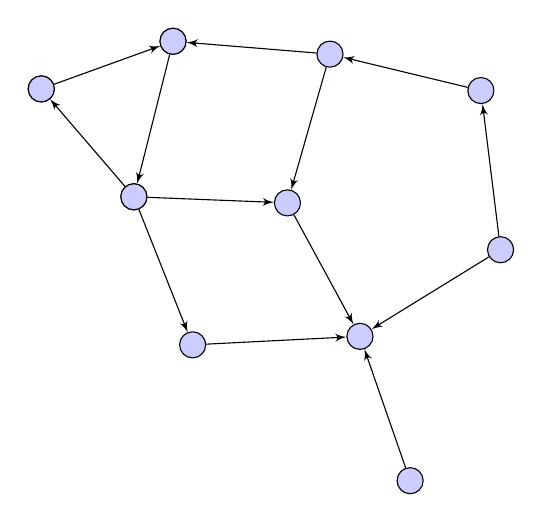
\begin{tikzpicture}[>=latex',line join=bevel,scale=0.7,every node/.style={scale=1,fill=blue!20}]
%%
  \node (10) at (107.78bp,-21.147bp) [draw,circle] { };
  \node (1) at (35.474bp,-65.695bp) [draw,circle] { };
  \node (3) at (-50.576bp,-70.065bp) [draw,circle] {};
  \node (2) at (61.283bp,-139.93bp) [draw,circle] {};
  \node (5) at (-1.8136bp,2.9476bp) [draw,circle] {};
  \node (7) at (20.058bp,79.448bp) [draw,circle] {};
  \node (9) at (97.672bp,60.723bp) [draw,circle] {};
  \visible<2->{\node (4) at (-80.797bp,6.0893bp) [draw,circle,fill=red] {};}
  \only<1>{\node (4a) at (-80.797bp,6.0893bp) [draw,circle] {};}
  \node (6) at (-60.664bp,86.061bp) [draw,circle,fill=red] {};
  \only<1>{\node (6a) at (-60.664bp,86.061bp) [draw,circle] {};}
  \node (8) at (-128.42bp,61.564bp) [draw,circle,fill=red] {};
  \only<1>{\node (8a) at (-128.42bp,61.564bp) [draw,circle] {};}
  \draw [->] (4) ..controls (-98.601bp,26.831bp) and (-103.44bp,32.466bp)  .. (8);
  \draw [->] (10) ..controls (104.25bp,7.41bp) and (102.62bp,20.665bp)  .. (9);
  \draw [->] (7) ..controls (-12.21bp,82.092bp) and (-17.962bp,82.563bp)  .. (6);
  \draw [->] (7) ..controls (12.354bp,52.502bp) and (9.0799bp,41.051bp)  .. (5);
  \draw [->] (2) ..controls (52.135bp,-113.62bp) and (48.405bp,-102.89bp)  .. (1);
  \draw [->] (10) ..controls (80.351bp,-38.045bp) and (71.978bp,-43.205bp)  .. (1);
  \draw [->] (4) ..controls (-48.846bp,4.8184bp) and (-43.811bp,4.6181bp)  .. (5);
  \draw [->] (3) ..controls (-16.455bp,-68.332bp) and (-8.9323bp,-67.95bp)  .. (1);
  \draw [->] (6) ..controls (-67.773bp,57.823bp) and (-70.987bp,45.055bp)  .. (4);
  \draw [->] (9) ..controls (66.898bp,68.148bp) and (61.149bp,69.535bp)  .. (7);
  \draw [->] (5) ..controls (11.585bp,-21.717bp) and (16.624bp,-30.995bp)  .. (1);
  \draw [->] (4) ..controls (-70.088bp,-20.897bp) and (-65.468bp,-32.538bp)  .. (3);
  \draw [->] (8) ..controls (-101.04bp,71.461bp) and (-97.613bp,72.701bp)  .. (6);
%
\end{tikzpicture}
\end{center}

\end{frame}


\begin{frame}[fragile]{Recurrence Set Example}
\begin{center}
\begin{columns}[c]
 \column{.3\textwidth}
  \begin{tabular}{c}
   \begin{lstlisting}[language=c,basicstyle=\normalsize]
while (x > 0) {
  x = x / 2;
  x = x + 1;
}
   \end{lstlisting}
  \end{tabular}
 \column{.3\textwidth}
 \pause
 \begin{gather*}
  x_0 = 2 \\
  S = \{ 2 \}
 \end{gather*}
\end{columns}
\end{center}

\pause

\begin{center}
\begin{columns}[c]
 \column{.3\textwidth}
  \begin{tabular}{c}
   \begin{lstlisting}[language=c,basicstyle=\normalsize]
while (x > 0) {
  x = x * 3;
}
   \end{lstlisting}
  \end{tabular}
 \column{.3\textwidth}
 \pause
 \begin{gather*}
  x_0 = 1 \\
  S = \{ x \mid (x \text{ mod } 2) = 1 \}
 \end{gather*}
\end{columns}
\end{center}

\end{frame}
% 
% \begin{frame}[fragile]{Nondeterminism and Non-Termination}
%  If the loop body contains some nondeterminism, we only require that for each $\red{S}$-state, there is
%  \emph{some} successor that is an $\red{S}$-state, rather than requiring that \emph{every} successor is an
%  $\red{S}$-state:
%   \begin{align*}
%   \exists \green{x_0} . & \red{S}(\green{x_0}) \\
%   \forall x . \red{S}(x) \Rightarrow & G(x) \\
%   \forall x \exists x' . \red{S}(x) \wedge B(x, x') \Rightarrow & \red{S}(x')
%  \end{align*}
% 
%  \vspace{1em}
%  
%  \pause
%  
% Our syntax does not allow us to existentially quantify over ground terms inside the universal.  To
% get around this, we Skolemise the formula, introducing a successor function $\blue{N}$ which picks
% out the next state for each $\red{S}$-state.
% \end{frame}

\begin{frame}{Second-Order Non-Termination}

\begin{block}{Skolemised Non-Termination Formula [SNT]}
 \[
 \exists \green{x_0}, \red{S}, \blue{N} . \forall x . \left ( \begin{array}{rl}
   \red{S}(\green{x_0}) \, \wedge & \\
   \red{S}(x) \Rightarrow & G(x) \, \wedge \\
   \red{S}(x) \Rightarrow & B(x, \blue{N}(x)) \wedge \red{S}(\blue{N}(x))
   \end{array} \right )
 \]
 \end{block}

 \vspace{1em}

This formula is satisfiable iff there exists a recurrence set $\blue{S}$ containing
an initial state $\red{x_0}$, with successor function $\blue{N}$, i.e. iff the loop
does not terminate for some input $\red{x_0}$.
\end{frame}

\subsection{Using Tautologies}

\begin{frame}{The Power of Tautologies}
 Our second-order solver works by trying to synthesise programs for each of the existentially quantified functions.

 \vspace{1em}

 This problem is NEXPTIME-hard, but in practice is quite fast if there is some short program that satisfies
 the constraints.

 \vspace{1em}

 However if the constraints are UNSAT, the solver will take a very long time to discover this.
\end{frame}

\begin{frame}{The Power of Tautologies}
 For a given loop, the formula \red{[CT]} is satisfiable iff the loop terminates and the formula \blue{[SNT]} is
 satisfiable iff it does not terminate.  Therefore, the formula
 \[
  \red{\text[CT]} \vee \blue{\text[SNT]}
 \]
 is satisfiable for \emph{every} loop.

 \vspace{1em}

 Since our solver produces witnesses to show that a formula is satisfiable, it will terminate with enough
 information to check whether the \red{[CT]} or \blue{[SNT]} disjunct has been satisfied.

 \vspace{1em}

 This allows us to avoid the expensive case of having to check an UNSAT formula.
\end{frame}

\section{Experiments}

\begin{frame}[fragile]{Fin}

\begin{center}
\includegraphics[width=.7\textwidth]{sloth.jpg}

\Huge
 Thank you!
\end{center}

\end{frame}


\end{document}
